\begin{frame}{Deux fonctionnalités réseaux utilisées dans SAVOIE : Isolation des flux}
\begin{block}{Quatre VLAN tagués sont utilisés}
\begin{itemize}
\item GESTION pour administrer les ESX et les SAN via un poste d'administration (LATANIA) \pause
\item vMOTION pour la migration des VM d'un ESX à un autre \pause
\item STOCKAGE pour les lectures et écritures sur le SAN \pause
\item SYSTEME sur lequel les VM applicatives serveurs communiquent avec les clients physiques \pause
\end{itemize}
\end{block}
\begin{block}{Pourquoi isoler les flux ?}
\begin{itemize}
    \item Préconisation de l'ANSSI \pause
    \item Allocation de ressources indépendantes et dédiées (Ex : Un VLAN GESTION a besoin de moins de ressources qu'un VLAN STOCKAGE)
\end{itemize}
\end{block}
 
\end{frame}

\begin{frame}{Deux fonctionnalités réseaux utilisées dans SAVOIE : Agrégation de liens réseaux}
\begin{block}{Avantages}
\begin{itemize}
\item Augmente la disponibilité réseaux en cas de perte d'un lien
\item Augmente le débit disponible pour une artère
\end{itemize}
\end{block}
\begin{block}{Inconvénients}
\begin{itemize}
\item Besoin d'un grand nombre de cartes Ethernet sur un ESX (8 dans SAVOIE, maximum possible simplement chez DELL)
\end{itemize}
\end{block} 
\begin{block}{Dans SAVOIE}
\begin{itemize}
\item Agrégation de 2 cartes pour GESTION, vMOTION, STOCKAGE et SYSTEME
\item Augmente le débit disponible pour une artère
\end{itemize}
\end{block}
\end{frame}

\begin{frame}{La Base}
    \begin{center}
    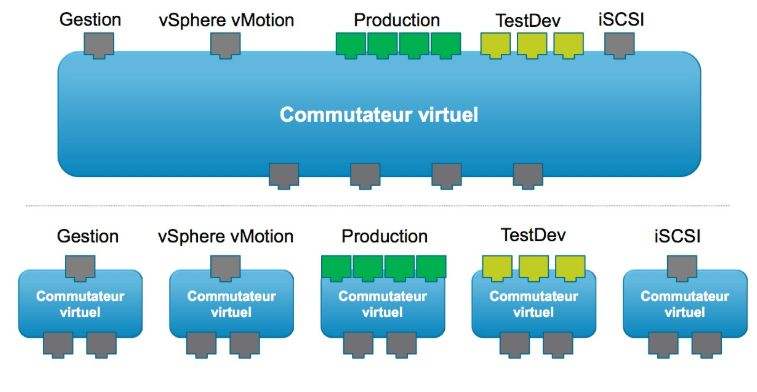
\includegraphics[width=300px]{Schemas/Commu.jpg}
    \end{center}
\end{frame}

\begin{frame}{Vu de l'ESX}
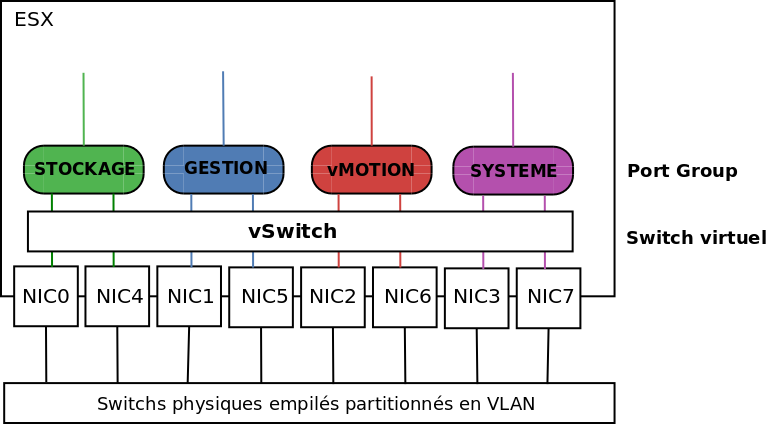
\includegraphics[width=300px]{Schemas/VLAN.png}
\end{frame}

\begin{frame}{Vu du SAN}
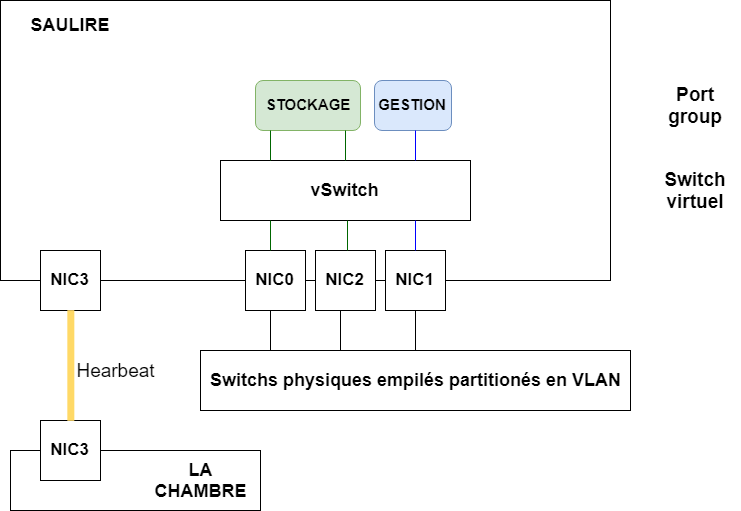
\includegraphics[width=300px]{Schemas/VuDuSan.png}
\end{frame}
